\chapter{Chain Attacks \small{\textsf{DRAFT}}}\label{chapter:attacks}

\section{Comparing Transactions and Blocks}

Now that we understand how blocks and transactions work, it is worth drawing parallels between the two.
\begin{center}
\begin{tabular}{ |c|c|c| }
  \hline
  & \textbf{Transaction} & \textbf{Block} \\
  \hline
  \textbf{Inductive base} & Coinbase & Genesis \\
  \hline
  \textbf{Inductive hypothesis} & Outpoint UTXO & Previous ID ($s$) \\
  \hline
  \textbf{Inductive step} & \makecell{Consuming produced UTXO \\ Signatures \\ Conservation laws} & \makecell{Proof of Work \\ Causality \\ Transactions} \\
  \hline
\end{tabular}
\end{center}

\section{Review of Ledger Virtues}
All fundamental use cases and proofs of security of blockchains are dependent on the following virtues being upheld.

\begin{itemize}
    \label{sec:liveness}
    \item \textbf{Liveness}: Honest transactions are included in all honest ledgers "soon".
    \label{sec:saftey}
    \item \textbf{Safety}: For any two honest ledgers $L_B$ and $L_D$ produced a ``sufficient time'' apart such that $L_D$ is fresher than $L_B$, $L_B$ must be a prefix of $L_D$. Note that ledgers may diverge for some time as long as blocks are mined within a network delay $\Delta$, but must satisfy this property upon reaching convergence opportunities (more on this in \hyperref[sec:mechanics]{Section 2.2}).
\end{itemize}

\section{Chain Virtues}
\subsection{Virtues}
The liveness and safety of ledgers directly follow from chain virtues. For this reason, we outline fundamental properties that chains must uphold.
\begin{itemize}
    \item \textbf{Common Prefix($k$)}:
        Honest parties agree on their chains with the exception of the last $k$ blocks. This chain virtue will be used to prove ledger safety(\hyperref[sec:saftey]{Section 1}).
        \begin{figure}[h]
        \centering
        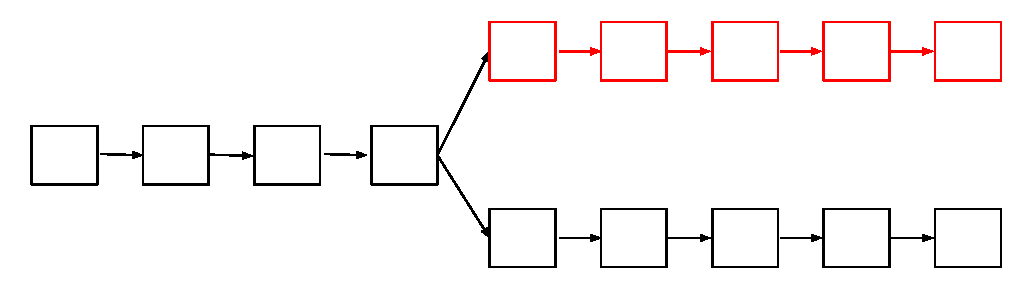
\includegraphics[width=\linewidth]{figures/commonprefix.pdf}
        \caption{These two chains satisfy the common prefix chain virtue with a $k$ of 6. The first 4 blocks of both chains are the honest parties common prefix.}
        \end{figure}
    \item \textbf{Chain Quality($\mu$)}: A sufficiently long chunk of the longest chain contains a $\mu > 0$ proportion of honest blocks.
    \begin{figure}[h]
    \centering
        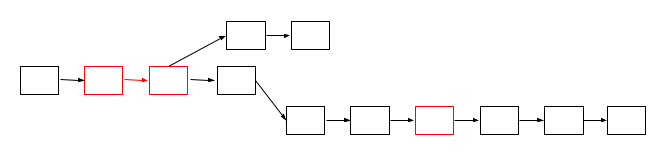
\includegraphics[width=\linewidth]{figures/chainquality.png}
        \caption{In this scenario the longest chain consists of 10 blocks. There are 3 blocks mined by an adversary and 7 honestly mined blocks in the longest chain. Hence, the chain quality $\mu$ of this chain is $70\%$. }
    \end{figure}
    \item \textbf{Chain Growth($\tau$)}: The chain adopted by honest parties will grow. Chain growth and chain quality will be used to prove the liveness virtue of ledgers(\hyperref[sec:liveness]{Section 1})

\end{itemize}

\subsection{Mechanics of Chain Divergence and Convergence}
Chain divergence happens when two or more blocks are mined at approximately the same time. When chain divergence happens, the honest node hash power is split up among multiple different chains. This is because there are multiple longest chains that the nodes can choose to extend. If blocks keep getting mined at the same time many chains can grow simultaneously. A convergence opportunity happens when exactly one block is mined with  period of silence of duration $\Delta$ before and after it. Honest parties move their hash power to extend the longest chain.
\begin{figure}
    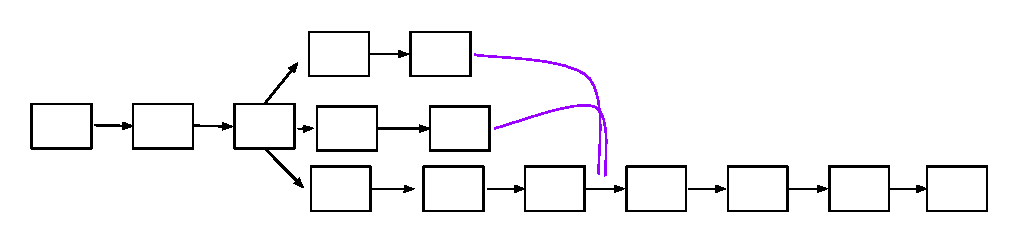
\includegraphics[width=\linewidth]{figures/divergence_convegence.pdf}
     \caption{In this scenario the chain diverges after the third block. This is because there were three blocks mined at about the same time. There is a convergence opportunity on the sixth block on the bottom chain. At this point honest nodes will switch over since they see the bottom chain is the new longest chain. The purple curved lines represent the honest parties switching over and adopting the new longest chain. }
    \label{sec:mechanics}
\end{figure}



\section{Network Attacks}
The attacks discussed in here are based on a strategy that gives rise to a "Nakamoto race".

Chain Quality is defined as the proportion of honestly mined blocks out of all mined blocks in a particular chain. A common conjecture is that Chain Quality can be approximated by the fraction of mining power that honest parties (however, future lectures will reveal that this is not the case).

In terms of chain virtues, the following attacks can break common prefix property and chain quality property if it were able to maintain the longest chain.

% Common prefix is broken if the adversary releases its chain to only a subset of nodes, thus making prefixes inconsistent until honest parties gossip amongst themselves. Chain quality is broken since a significant portion of the released chain is mined by the adversary.  Virtue \#2 (chain growth) is upheld as long as there are any honest participants mining that force the adversarial chain to grow.
\subsection{Nakamoto Attack}
The strategy of Nakamoto attack involves the adversary mining a competing chain in silent, withholding constituent blocks for as long as desired (often when the target adversarial transactions are buried $k$ blocks deep for instant confirmation). Therefore, since honest miners are unaware of that private adversarial chain, they continue extending the longest honest chain.
The adversary is, in effect, "racing" to construct a chain longer than the longest honest chain. If the private chain is longer that the honest chain, adversary can release the private chain. In such case, honest participants have to switch and extend the adversarial chain since it is the new longest chain. Thus, this adversarial chain replaces the honest chain. If the honest parties switch chains by reverting more than $k$ blocks, then the adversary has broken the Common Prefix property.

This attack is unlikely to succeed for a minority adversary. Consider the situation where the adversary and the honest parties begin mining at a particular block. Breaking Common Prefix requires that the honest parties mine a chain $k$ blocks long after that common block, while the adversary also mines $k$ or more blocks after the common block. As $k$ is chosen to be a somewhat large value, it will take time for the honest parties to mine $k$ blocks. Given that this span of time will be sufficiently large, the number of adversarially mined blocks will be fewer than the honest convergence opportunities within that timespan. If this is the case, the adversary cannot win.

\subsection{Fan-out Attack}
\begin{figure}
  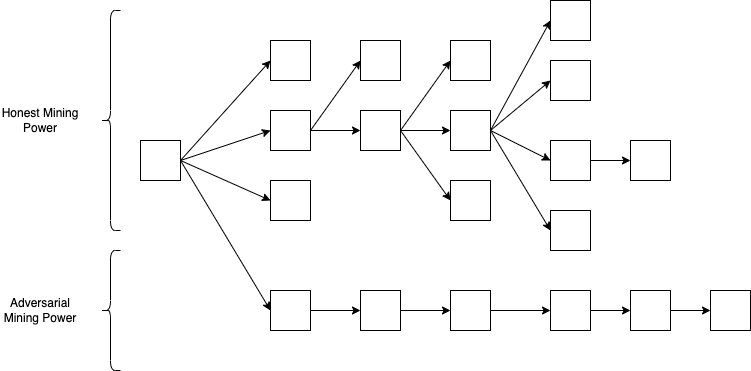
\includegraphics[width=\linewidth]{figures/fan_out.png}
  \caption{A fan-out attack where an adversary who does not hold majority hashing power can still produce the longest chain due to honest mining power being wasted. Displays a drawback of having infrequent convergence opportunities.}
  \label{fig:fan_out}
\end{figure}

This type of attack is unique in that it is more due to a fault of the network rather than an exploit from an adversary. Networks are susceptible to fan-out attacks when convergence opportunities are rare.

Infrequent convergence opportunities lead to honest nodes frequently working on competing chains, thus making the chain "fan out" as shown in \ref{fig:fan_out}. All but one of these competing branches are eventually thrown out, leading to the honest mining power being wasted. An adversary, on the other hand, can coordinate its attack to build on a single withheld chain, winning the race even without having majority hashing power. This is the reason why we do not want fast chains where the target is easily attainable.

\subsection{Majority Adversary Attack}
Now if the adversary held the majority of mining power in a network, all she needs to do is to mine a secret chain, which can be released at any time due to having more compute power. What properties can adversary break if she holds majority of the network hash power?

Clearly, she can violate the Common Prefix property as was mentioned earlier. If honest parties agree on the longest chain containing some block $B_m$, she mines a secret chain extending from the previous block $B_{m-1}$. Once the longest chain has $k$ or more blocks after $B_m$, she releases her secret chain to some of the honest miners. Since the adversarial chain is longer than the honest chain, these honest miners adopt the adversarial chain.

Additionally, an adversary with majority hash power can break Chain Quality as follows. If a block $B_m$ is mined by an honest miner, she creates a new longest chain extending the block $B_{m-1}$. Thus, the block $B_m$ is ``replaced" by a new block mined by the adversary. We will discuss this attack in more details in the next lecture.

However, in such attacks Chain Growth is upheld as long as there are any honest participants mining that force the adversarial chain to grow.
